
\chapter[Dạng bài: Xác định điểm dao động với biên độ thỏa điều kiện cho trước]{Dạng bài: Xác định điểm dao động với biên độ thỏa điều kiện cho trước}
\section{Lý thuyết}
\subsection{Dao động của một điểm trong vùng giao thoa}

Gọi M là một điểm trong vùng giao thoa, lần lượt cách $\text{S}_1$, $\text{S}_2$ những khoảng $d_1=\text{S}_1\text{M}$ và $d_2=\text{S}_2\text{M}$. Chọn gốc thời gian sao cho phương trình dao động của hai nguồn là
\begin{equation*}
	u_{\text{S}_1}=u_{\text{S}_2}=A\cos\dfrac{2\pi t}{T}.
\end{equation*}
\begin{center}
	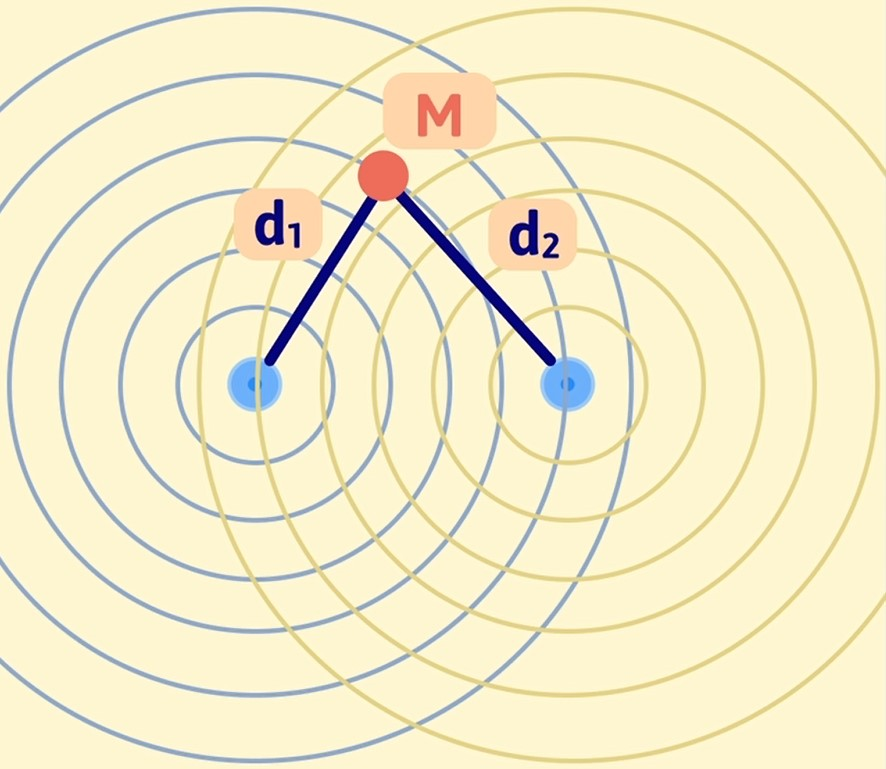
\includegraphics[scale=0.3]{../figs/VN12-PH-11-A-007-1-V2-0.JPG}
\end{center}
\subsubsection{Phương trình dao động tại M}
\begin{equation*}
	u_{\text{M}}=2A\cos\dfrac{\pi(d_2-d_1)}{\lambda}\cos 2\pi \left(\dfrac{t}{T}-\dfrac{d_1+d_2}{2\lambda}\right)$$
	$$\Rightarrow u_{\text{M}}=2A\cos\dfrac{\pi(d_2-d_1)}{\lambda}\cos \left(\omega t-\dfrac{\pi (d_1+d_2)}{\lambda}\right).
\end{equation*}

Vậy, dao động của phần tử M là dao động điều hòa cùng \bltext{chu kì} với hai nguồn.

\subsubsection{Biên độ dao động tại M}
\begin{equation*}
	A_{\text{M}}=\left|2A\cos\dfrac{\pi(d_2-d_1)}{\lambda}\right|.
\end{equation*}
\subsection{Vị trí cực đại và cực tiểu giao thoa}
\subsubsection{Trường hợp hai nguồn lệch pha nhau bất kì}
\begin{itemize}
	\item Vị trí cực tiểu giao thoa:
	
	\begin{equation*}
		d_2-d_1 = \left(k+ \dfrac{1}{2}\right) \lambda + \dfrac{\varphi_2 - \varphi_1}{2\pi} \lambda,\quad k \in \mathbb{Z}.
	\end{equation*}
	\item Vị trí cực đại giao thoa:
	\begin{equation*}
		d_2-d_1 = k\lambda + \dfrac{\varphi_2 - \varphi_1}{2\pi} \lambda,\quad k \in \mathbb{Z}.
	\end{equation*}
\end{itemize}
\subsubsection{Trường hợp hai nguồn cùng pha}
\begin{itemize}
	\item Vị trí cực tiểu giao thoa:
	
	\begin{equation*}
		d_2-d_1 = \left(k'+ \dfrac{1}{2}\right) \lambda,\quad k' \in \mathbb{Z}.
	\end{equation*}
	
	\item Vị trí cực đại giao thoa:
	
	\begin{equation*}
		d_2-d_1 = k'\lambda,\quad k' \in \mathbb{Z}.
	\end{equation*}
\end{itemize}	
\subsubsection{Trường hợp hai nguồn ngược pha}
\begin{itemize}
	\item Vị trí cực tiểu giao thoa:
	\begin{equation*}
		d_2-d_1 = k'\lambda,\quad k' \in \mathbb{Z}.
	\end{equation*}
	
	\item Vị trí cực đại giao thoa:
	
	\begin{equation*}
		d_2-d_1 = \left(k'+ \dfrac{1}{2}\right) \lambda,\quad k' \in \mathbb{Z}.
	\end{equation*}
	
\end{itemize}
\section{Mục tiêu bài học - Ví dụ minh họa}
\begin{dang}{Xác định được số điểm, số đường cực đại, cực tiểu trên đoạn thẳng nối hai nguồn}
	\ppgiai{Dạng bài này thường yêu cầu tìm các điểm có biên độ thỏa điều kiện cho trước (cực đại hoặc cực tiểu) nằm giữa hai điểm M và N trong vùng giao thoa. 
		
		\textbf{Hai điểm M và N nằm cùng phía so với đường thẳng nối hai nguồn}
		
		\begin{description}
			\item[Bước 1:] Giả sử điểm P bất kì thuộc MN thỏa mãn yêu cầu bài toán (là điểm cực đại hoặc cực tiểu), cách hai nguồn các đoạn tương ứng là $d_1$ và $d_2$.
			\item [Bước 2:] Tính hiệu khoảng cách $\Delta d=d_2-d_1$ từ hai nguồn đến điểm đó.
			
			Cách tính: từ độ lệch pha của hai sóng truyền từ hai nguồn đến P (P dao động với biên độ cực đại khi độ lệch pha là $k2\pi$, P dao động với biên độ cực tiểu khi độ lệch pha là $\pi +k2\pi$ với $k \in \mathbb{Z}$), áp dụng các công thức ở phần lý thuyết, ta suy ra được hiệu khoảng cách $\Delta d$ là biểu thức phụ thuộc $k$.
			\item [Bước 3:] Cho P chạy trong MN ta sẽ tìm được vùng giá trị của $\Delta d$, từ đó suy ra vùng giá trị của $k$. Số giá trị của $k$ tìm được chính là số điểm dao động với biên độ cực đại hoặc cực tiểu cần tính.
		\end{description}
		\luuy{Trường hợp các điểm M hoặc N (hoặc cả hai điểm) nằm trên đường thẳng nối hai nguồn, ta cũng sử dụng cùng cách làm như trên. }
		\textbf{Hai điểm M và N nằm khác phía so với đường thẳng nối hai nguồn}
		
		Khi M và N ở khác phía so với đường thẳng nối hai nguồn, MN sẽ cắt đường thẳng nối hai nguồn tại điểm Q. Ta sẽ tìm số điểm dao dộng cực đại hoặc cực tiểu trên từng đoạn MQ, QN theo trường hợp 2.1, sau đó cộng lại để tìm số điểm cực đại hoặc cực tiểu trên cả đoạn MN.
		
		\textbf{Nhận xét:}
		
		\begin{itemize}
			\item Nếu hai nguồn cùng pha.
			
			+ Số đường dao động cực đại đi qua đoạn thẳng nối hai nguồn là số giá trị nguyên của $k$ thỏa mãn: 
			\begin{equation*}
				\dfrac{-\text{AB}}{\lambda} < k < \dfrac{\text{AB}}{\lambda}.
			\end{equation*} 
			+ Số đường dao động cực tiểu đi qua đoạn thẳng nối hai nguồn là số giá trị nguyên của $k$ thỏa mãn: 
			\begin{equation*}
				\dfrac{-\text{AB}}{\lambda} -\dfrac{1}{2} < k < \dfrac{\text{AB}}{\lambda} -\dfrac{1}{2}.
			\end{equation*} 
			\item Nếu hai nguồn ngược pha.
			
			+ Số đường dao động cực đại đi qua đoạn thẳng nối hai nguồn là số giá trị nguyên của $k$ thỏa mãn: 
			\begin{equation*}
				\dfrac{-\text{AB}}{\lambda} -\dfrac{1}{2} < k < \dfrac{\text{AB}}{\lambda} -\dfrac{1}{2}.
			\end{equation*} 
			+ Số đường dao động cực tiểu đi qua đoạn thẳng nối hai nguồn là số giá trị nguyên của $k$ thỏa mãn: 
			\begin{equation*}
				\dfrac{-\text{AB}}{\lambda} < k < \dfrac{\text{AB}}{\lambda}.
			\end{equation*} 
			
	\end{itemize}}
	\viduii{3}{Tại hai điểm A, B trên mặt chất lỏng cách nhau 10 cm có hai nguồn phát sóng theo phương thẳng đứng với các phương trình: $u_1 = \text{0,2} \cos 50 \pi t \ \text{cm}$ và $u_2 = \text{0,2} \cos (50 \pi t + \pi)\ \text{cm}$. Vận tốc truyền sóng là $\text{0,5}\ \text{m/s}$. Coi biên độ sóng không đổi. Xác định số điểm dao động với biên độ cực đại trên đoạn thẳng AB.
	}
	{
		\begin{center}
			\textbf{Hướng dẫn giải}
		\end{center}
		
		\begin{itemize}
			\item A, B là hai nguồn dao động ngược pha nên số điểm dao động cực đại là số nguyên của $k$ thỏa mãn:
			\begin{equation*}
				\dfrac{-\text{AB}}{\lambda} -\dfrac{1}{2} < k < \dfrac{\text{AB}}{\lambda} -\dfrac{1}{2}.
			\end{equation*}
			\item Theo đề bài $\lambda =\dfrac{v}{f}= 2\ \text{cm}$. Từ đó: 
			\begin{equation*}
				-\dfrac{10}{2} -\dfrac{1}{2} < k < \dfrac{10}{2} -\dfrac{1}{2} \Rightarrow -\text{5,5} < k < \text{4,5}.
			\end{equation*}
			\item Vậy có 10 điểm dao động với biên độ cực đại.
			
		\end{itemize}
	}
	\viduii{3}
	{Ở mặt thoáng của một chất lỏng có hai nguồn sóng kết hợp A và B cách nhau $\SI{20}{cm}$, dao động cùng pha theo phương thẳng đứng với tần số là $\SI{20}{Hz}$. Biết tốc độ truyền sóng trên mặt chất lỏng là $\SI{30}{cm/\second}$. Số điểm dao động với biên độ cực đại trên đoạn AB là
		\begin{mcq}(4)
			\item 25.
			\item 26.
			\item 27.
			\item 28.
	\end{mcq}}
	{\begin{center}
			\textbf{Hướng dẫn giải}
		\end{center}
		
		Vì AB là nguồn nên số điểm dao động với biên độ cực đại trên đoạn AB thỏa mãn:
		$$\Delta d_\text{B}< {d_2}-{d_1}< d_\text{A};$$
		trong đó:
		\begin{itemize}
			\item
			$ \Delta d_\text{A}=\text{AB}-\text{AA}=\SI{20}{cm}-0=\SI{20}{cm}$;
			\item
			$ \Delta d_\text{B}=\text{BB}-\text{BA}=0-\SI{20}{cm}=-\SI{20}{cm}$,
			\item
			$d_2-d_1=k\lambda=k\dfrac{v}{f}=k\cdot\dfrac{\SI{30}{cm/\second}}{\SI{20}{Hz}}=\SI{1.5}{}k\,\text{cm}$.
		\end{itemize}
		
		Do đó:
		$$ -\SI{20}{}<\SI{1.5}{}k< \SI{20}{}$$ $$\Rightarrow -\SI{13.3}{}< k < \SI{13.3}{}$$  $$\Rightarrow k= -13,-12,-11,... 11,12,13.$$
		
		Vậy có 27 điểm dao động với biên độ cực đại trên đoạn AB.
		
		\textbf{Đáp án: C.}
	}
	\viduii{4}
	{
		Trên mặt một chất lỏng, có hai nguồn sóng kết hợp $\text{O}_1, \text{O}_2$ cách nhau $l=24\ \text{cm}$, dao động theo cùng một phương với phương trình $u_{\text{O}_1}=u_{\text{O}_2} = A \cos \omega t $ ($t$ tính bằng $s$, $A$ tính bằng $\text{mm}$). Khoảng cách ngắn nhất từ trung điểm O của $\text{O}_1 \text{O}_2$ đến các điểm nằm trên đường trung trực của $\text{O}_1\text{O}_2$ dao động cùng pha với O bằng $q=9\ \text{cm}$. Số điểm dao động với biên độ bằng biên độ của O trên đoạn $\text{O}_1\text{O}_2$ là
		\begin{mcq}(4)
			\item 18.
			\item 16.
			\item 20.
			\item 14.
		\end{mcq}
	}{
		\begin{center}
			\textbf{Hướng dẫn giải}
			
			\vspace*{1em}
			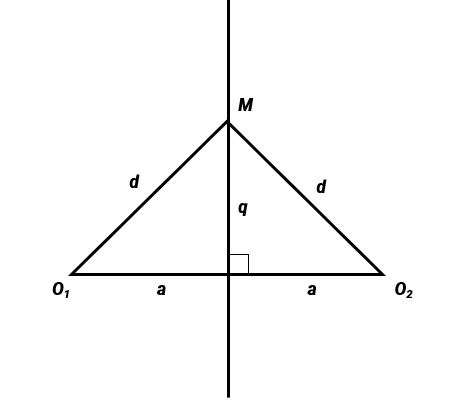
\includegraphics[scale=0.9]{../figs/VN12-PH-11-A-007-1-V2-1.JPG}
		\end{center}
		\begin{itemize}
			\item Vì hai nguồn dao động cùng pha nên các điểm thuộc trung trực dao động với biên độ cực đại (điểm O dao động với biên độ cực đại) nên để tìm số điểm dao động với biên độ cực đại trên $\text{O}_1\text{O}_2$ (không kể O).
			\item Phương trình dao động tại một điểm khi có giao thoa:
			\begin{equation*}
				u =2A \cos \left (\pi \dfrac {d_1-d_2}{\lambda}\right) \cos \left(\omega t -\pi \dfrac{d_1+d_2}{\lambda}\right).
			\end{equation*}
			\item Phương trình dao động tại O:
			\begin{equation*}
				u_{\text{O}} = 2A \cos \left(\omega t - \dfrac{2\pi a}{\lambda}\right)\ (\text{với } l=2a).
			\end{equation*}
			\item Phương trình dao động tại M:
			\begin{equation*}
				u_{\text{M}} = 2A \cos \left(\omega t - \dfrac{2\pi d}{\lambda}\right).
			\end{equation*}
			\item Độ lệch pha của M so với O:
			\begin{equation*}
				\Delta \varphi = \dfrac{2\pi}{\lambda} (d-a).
			\end{equation*}
			\item Do M dao động cùng pha với O:
			\begin{equation*}
				\Delta \varphi = \dfrac{2\pi}{\lambda} (d-a)=2k\pi \Rightarrow d-a=k\lambda.
			\end{equation*}
			\item Điểm M gần O nhất thì $k=1$, nên:
			\begin{equation*}
				\Rightarrow \lambda = d-a =\sqrt {a^2+q^2} - a =\sqrt {12^2+9^2} -12 =3\ \text{cm}.
			\end{equation*}
			\item Số cực đại:
			\begin{equation*}
				-\dfrac{l}{\lambda} \leq k \leq \dfrac{l}{\lambda} \Rightarrow -8 \leq k \leq 8.
			\end{equation*}
			\item Có 17 cực đại trên $\text{O}_1\text{O}_2$ (kể cả O).
			\item Vậy có 16 điểm dao động với biên độ bằng biên độ của điểm O.
		\end{itemize}
		
		\textbf{Đáp án: B.}
	}
	
\end{dang}
\begin{dang}{Xác định được số điểm, số đường cực đại, cực tiểu nằm ngoài đoạn thẳng\\ nối hai nguồn}
	\viduii{3}{Người ta tạo ra giao thoa sóng trên mặt nước hai nguồn A, B dao động với phương trình $u_\text{A}=u_\text{B}=5\cos10\pi t\, \text{cm}$. Tốc độ truyền sóng trên mặt nước là $\SI{20}{cm/\second}$. Một điểm N trên mặt nước với $\text{AN}-\text{BN}=-\SI{10}{cm}$ nằm trên đường cực đại hay cực tiểu thứ mấy, kể từ đường trung trực của AB?
		\begin{mcq}(2)
			\item Cực đại thứ 3 về phía A.
			\item Cực tiểu thứ 3 về phía A.
			\item Cực đại thứ 4 về phía B.
			\item Cực tiểu thứ 4 về phía B.
		\end{mcq}
	}
	{
		\begin{center}
			\textbf{Hướng dẫn giải}
		\end{center}
		
		Bước sóng là
		$$\lambda=\dfrac{v}{f}=\dfrac{2\pi v}{\omega}=\dfrac{2\pi \cdot\SI{20}{cm/\second}}{\xsi{10\pi}{\radian/\second}}=\SI{4}{cm}.$$ 
		
		Ta có: $$\text{AN}-\text{BN}=-\SI{10}{cm}=2,5\lambda.$$
		
		Vì hai nguồn cùng pha nên trung trực AB là một cực đại giao thoa.
		
		$\Rightarrow$ N nằm ở cực tiểu thứ 3 về phía A.
		
		\textbf{Đáp án: B.}
	}
	
	\viduii{3}
	{
		Người ta tạo ra giao thoa sóng trên mặt nước hai nguồn A,B dao động với phương trình $u_\text{A}=5\cos10\pi t\, \text{cm}$ và $u_\text{B}=5\cos(10\pi t+\pi)\, \text{cm}$. Tốc độ truyền sóng trên mặt nước là $\SI{20}{cm/\second}$. Một điểm N trên mặt nước với $\text{AN}-\text{BN}=-\SI{10}{cm}$ nằm trên đường cực đại hay cực tiểu thứ mấy, kể từ đường trung trực của AB?
		\begin{mcq}(2)
			\item Cực đại thứ 3 về phía A.
			\item Cực tiểu thứ 3 về phía A.
			\item Cực đại thứ 4 về phía B.
			\item Cực tiểu thứ 4 về phía B.
		\end{mcq}
	}{
		\begin{center}
			\textbf{Hướng dẫn giải}
		\end{center}
		
		Bước sóng là
		$$\lambda=\dfrac{v}{f}=\dfrac{2\pi v}{\omega}=\dfrac{2\pi \cdot\SI{20}{cm/\second}}{\xsi{10\pi}{\radian/\second}}=\SI{4}{cm}.$$ 
		
		Ta có: $$\text{AN}-\text{BN}=-\SI{10}{cm}=2,5\lambda.$$
		
		Vì hai nguồn ngược pha nên trung trực AB là một cực tiểu giao thoa.
		
		$\Rightarrow$ N nằm ở cực đại thứ 3 về phía A.
		
		\textbf{Đáp án: A.}
	}
\end{dang}
\begin{dang}{Xác định được số điểm, số đường cực đại, cực tiểu trên đường tròn, elip, hình chữ nhật, hình vuông, $\ldots$}
	\viduii{3}{Ở mặt thoáng của một chất lỏng có hai nguồn kết hợp A, B cách nhau 10 cm, dao động theo phương thẳng đứng với phương trình lần lượt là $u_{\text{A}} = 3 \cos \left(40\pi t + \dfrac{\pi}{6}\right)\ \text{cm}$; $u_{\text{B}}= 4\cos \left (40\pi t +\dfrac{2\pi}{3}\right)\ \text{cm}$. Cho biết tốc độ truyền sóng là 40 cm/s. Một đường tròn có tâm là trung điểm của AB, nằm trên mặt nước, có bán kính $R$ với $R=4\ \text{cm}$. Số điểm dao động với biên độ 5 cm có trên đường tròn là
		\begin{mcq}(4)
			\item 30.
			\item 32.
			\item 34.
			\item 36.
		\end{mcq}
	}
	{
		\begin{center}
			\textbf{Hướng dẫn giải}
			
			\vspace*{1em}
			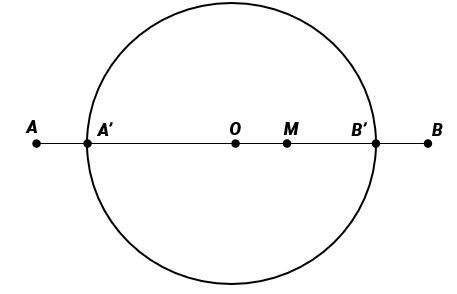
\includegraphics[scale=0.7]{../figs/VN12-PH-11-A-007-1-V2-2.JPG}
		\end{center}
		
		Các dữ kiện vận tốc truyền sóng và tần số (suy ra từ tần số góc trong phương trình sóng) cho phép tính giá trị bước sóng 
		\begin{equation*}
			\lambda = \dfrac{v}{f} = 2\ \text{cm}.
		\end{equation*}
		
		Gọi A' và B' là giao điểm của đường tròn với đường nối AB, xét điểm M trên đoạn A'B' với các khoảng cách đến nguồn $d_1=\text{AM}$ và $d_2= BM$. Sóng truyền từ A đến M có phương trình 
		\begin{equation*}
			u_{\text{AM}} = 3\cos \left(10\pi t +\dfrac{\pi}{6} - \dfrac{2\pi d_1}{\lambda}\right) = 3 \cos \left(10\pi t +\dfrac{\pi}{6} - \pi d_1\right)
		\end{equation*}
		Sóng truyền từ B đến M có phương trình
		\begin{equation*}
			u_{\text{BM}} = 4 \cos \left (10 \pi t + \dfrac{2\pi}{3} - \dfrac{2\pi d_2}{\lambda}\right) = 4 \cos \left (10 \pi t + \dfrac{2\pi}{3} - \dfrac{2\pi (10-d_1)}{\lambda}\right)
		\end{equation*}
		\begin{equation*}
			= 4 \cos \left (10 \pi t + \dfrac{2\pi}{3} - \pi d_1 -10\pi\right) = 4 \cos \left (10\pi t +\dfrac{2\pi}{3} + \pi d_1 \right).
		\end{equation*}
		Phương trình sóng tổng hợp $u_{\text{M}} =u_{\text{AM}}+ u_{\text{BM}} $ có biên độ bằng 5 cm khi $u_{\text{AM}}$ và $u_{\text{BM}}$ vuông pha với nhau 
		\begin{equation*}
			\dfrac{2\pi}{3} + \pi d_1 - \left(\dfrac{\pi}{6} - \pi d_1\right) = \dfrac{\pi}{2} +k\pi \Rightarrow d_1 =\dfrac{k}{2}.
		\end{equation*}
		Cho M chạy trên đoạn A'B', ta có điều kiện của khoảng cách $d_1$
		\begin{equation*}
			1 \leq d_1 = \dfrac{k}{2} \leq 9 \Rightarrow 2 \leq k \leq 18.
		\end{equation*}
		có 17 giá trị $k$ nguyên thỏa mãn. 
		
		Như vậy trên đoạn A'B' có 17 điểm dao động với biên độ 5 cm trong đó có điểm A' và B'. Suy ra trên đường tròn tâm O bán kính $R=4\ \text{cm}$ có 32 điểm dao động với biên độ $5\ \text{cm}$.
		
		\textbf{Đáp án: B.}
	}
	
	\viduii{3}
	{
		Ở mặt thoáng của một chất lỏng có hai nguồn sóng kết hợp A và B cách nhau $\SI{20}{cm}$, dao động cùng pha theo phương thẳng đứng với tần số là $\SI{20}{Hz}$. Biết tốc độ truyền sóng trên mặt chất lỏng là $\SI{30}{cm/\second}$. Xét hình vuông AMNB thuộc mặt thoáng chất lỏng. Số điểm dao động với biên độ cực đại trên đoạn MN là
		\begin{mcq}(4)
			\item 11.
			\item 12.
			\item 13.
			\item 14.
		\end{mcq}
	}{
		\begin{center}
			\textbf{Hướng dẫn giải}
			
			\vspace*{1em}
			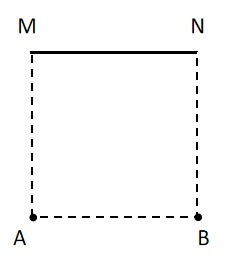
\includegraphics[scale=0.8]{../figs/VN12-PH-11-A-007-1-V2-3.jpg}
		\end{center}
		Số điểm dao động với biên độ cực đại trên đoạn MB thỏa mãn:
		$$\Delta d_\text{N}\leq {d_2}-{d_1}\leq d_\text{M};$$
		trong đó:
		\begin{itemize}
			\item
			$ \Delta d_\text{N}=\text{NB}-\text{NA}=\text{NB}-\text{NB}\sqrt{2}\approx-\SI{8.3}{cm}$;
			\item
			$ \Delta d_\text{M}=\text{MB}-\text{MA}=\text{MA}\sqrt{2}-\text{MA}\approx\SI{8.3}{cm}$.
			\item
			$d_2-d_1=k\lambda=k\dfrac{v}{f}=k\cdot\dfrac{\SI{30}{cm/\second}}{\SI{20}{Hz}}=\SI{1.5}{}k\,\text{cm}$.
		\end{itemize}
		
		Do đó:
		$$ -\SI{8.3}{}\le \SI{1.5}{}k\le \SI{8.3}{}$$ $$\Rightarrow -\SI{5.5}{}\le k\le \SI{5.5}{}$$  $$\Rightarrow k= -5,-4,-3,....3,4,7,5.$$
		
		Vậy có 11 điểm dao động với biên độ cực đại trên đoạn MN.
		
		\textbf{Đáp án: A.}
	}
	\viduii{3}
	{Ở mặt thoáng của một chất lỏng có hai nguồn sóng kết hợp A và B cách nhau $\SI{20}{cm}$, dao động cùng pha theo phương thẳng đứng với tần số là $\SI{20}{Hz}$. Biết tốc độ truyền sóng trên mặt chất lỏng là $\SI{30}{cm/\second}$. Xét hình vuông AMNB thuộc mặt thoáng chất lỏng. Số điểm dao động với biên độ cực đại trên đoạn MB là
		\begin{mcq}(4)
			\item 17.
			\item 18.
			\item 19.
			\item 20.
	\end{mcq}}
	{\begin{center}
			\textbf{Hướng dẫn giải}
			
			\vspace*{1em}	
			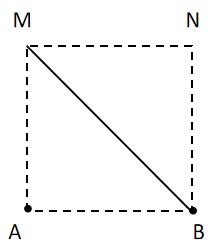
\includegraphics[scale=0.8]{../figs/VN12-PH-11-A-007-1-V2-4.jpg}
		\end{center}
		
		Số điểm dao động với biên độ cực đại trên đoạn MB thỏa mãn:
		$$\Delta d_\text{B}<{d_2}-{d_1}\le d_\text{M};$$
		trong đó:
		\begin{itemize}
			\item
			$ \Delta d_\text{M}=\text{MB}-\text{MA}=\text{MA}\sqrt{2}-\text{MA}\approx\SI{8.3}{cm}$;
			\item
			$ \Delta d_\text{B}=\text{BB}-\text{BA}=0-\SI{20}{cm}=-\SI{8.3}{cm}$;
			\item
			$d_2-d_1=k\lambda=k\dfrac{v}{f}=k\cdot\dfrac{\SI{30}{cm/\second}}{\SI{20}{Hz}}=\SI{1.5}{}k\,\text{cm}$.
		\end{itemize}
		Do đó:
		$$ -\SI{20}{}<\SI{1.5}{}k\leq \SI{8.3}{}$$ $$\Rightarrow -\SI{13.3}{}<k\leq \SI{4.4}{}$$  $$\Rightarrow k= -13,-12,-11,....1,2,3,4.$$
		
		Vậy có 18 điểm dao động với biên độ cực đại trên đoạn MB.
		
		\textbf{Đáp án: B.}
	}
\end{dang}